% !TeX program = pdflatex
% Select the legacy text encoding before IEEEtran loads its Times fonts.
% This also prevents TU/ptm font substitution when compiling with XeLaTeX.
\RequirePackage[T1]{fontenc}
\documentclass[conference]{IEEEtran}
% Suppress build timestamps and engine metadata from the release PDF.
\ifdefined\pdfinfoomitdate\pdfinfoomitdate=1\fi
\ifdefined\pdftrailerid\pdftrailerid{}\fi
\ifdefined\pdfsuppressptexinfo\pdfsuppressptexinfo=15\fi
% IEEEtran.cls is the unchanged class distributed on the SGC 2026 website.
% Preserve the official margins, fonts, column widths, and line spacing.
\usepackage{cite}
\usepackage{amsmath,amssymb,amsfonts}
\usepackage{graphicx}
\usepackage{textcomp}
\usepackage{booktabs}
\usepackage{array}
\usepackage{url}
\usepackage{balance}
\usepackage[hidelinks]{hyperref}
\usepackage[all]{hypcap}
\hypersetup{pdftitle={Incremental Value of Weather and Calendar Inputs in Hour-Ahead Load Forecasting},pdfsubject={Retrospective input comparisons for hour-ahead load forecasting}}
\graphicspath{{figures/}}
\newcommand{\full}{\textsc{Full}}
\newcommand{\proxy}{\textsc{Proxy}}
\newcommand{\mdw}{\overline{\mathrm{WAPE}}}
\newcommand{\degc}{\ensuremath{^{\circ}\mathrm{C}}}
\begin{document}

\title{Incremental Value of Weather and Calendar Inputs in Hour-Ahead Load Forecasting}
% Author metadata intentionally omitted pending confirmation.
\author{}

\maketitle

\begin{abstract}
Recent load may already encode information carried by weather and recurring schedules. We assess the incremental forecasting value of explicit weather, calendar, and thermal inputs using Ridge-ARX, XGBoost, and the Time-series Dense Encoder (TiDE) for hour-ahead load forecasting in a city in Iran. All seven input conditions share the same 168-hour history and preprocessing and are evaluated in two chronological windows. Removing weather lowers cold-window mean daily weighted absolute percentage error by 2.45, 0.97, and 0.79 percentage points for Ridge, XGBoost, and TiDE, respectively. Warm-window effects differ: removal helps Ridge, harms XGBoost, and gives an initialization-sensitive TiDE result. Cold peak-magnitude error improves for Ridge and XGBoost but worsens for TiDE. Agreement across model families therefore depends on both the evaluation period and the forecasting objective. These retrospective results support checking input value across models, periods, and average and peak errors; they do not identify causal effects on electricity demand.
\end{abstract}

\begin{IEEEkeywords}
load forecasting, weather inputs, feature ablation, model comparison, peak demand, temporal evaluation
\end{IEEEkeywords}

\section{Introduction}
At an hour-ahead horizon, recent load contains information about weather, operating schedules, and recurring demand patterns. The additional forecasting value of explicit weather and calendar variables is therefore conditional on this history. Assessing that value requires comparisons that distinguish input representation, information available at the forecast origin, and the performance criterion relevant to the application.

Existing work gives several reasons to avoid assuming that more inputs will improve accuracy. Fan and Hyndman selected calendar, demand, and temperature terms by forecasting performance rather than statistical relevance alone \cite{fan2012}. Pinheiro \emph{et al.} evaluated load lags and calendar refinements as distinct additions to a weather-aware model \cite{pinheiro2023}. At the low-voltage level, Haben \emph{et al.} found that adding observed or forecast temperature did not improve the average accuracy of their seasonal autoregressive model \cite{haben2019}. ERCOT experiments likewise showed that the preferred combination of weather and time features depended on model capacity \cite{yang2024}. These results do not establish that weather is unimportant; they show why its predictive value must be measured conditionally.

How temperature is represented also matters. Wang \emph{et al.} studied lagged hourly temperatures and daily moving averages, showing that useful temperature memory can differ across load zones and hours \cite{wang2016}. An operational Spanish study improved a fixed forecasting system through temperature preprocessing, threshold selection, and lag selection \cite{candela2022}. Cai \emph{et al.} combined recent and previous-day weather through Fisher-information weighting \cite{cai2018}. Humidity-related heat-stress indicators have improved models of monthly residential summer demand in many US states \cite{maia2020}, although that evidence does not directly determine the value of raw humidity at an hourly horizon. These studies motivate testing thermal and humidity inputs without presupposing a useful memory length or a transferable effect size.

An importance score does not directly establish the value of an input under retraining. Accuracy losses after input removal can differ from learned variable-selection weights \cite{nicola2026}; perturbation effects depend on the event examined \cite{gurses2022}, and temporal dependence complicates post-hoc attribution \cite{baur2024}. These distinctions motivate evaluating models trained without the information concerned.

Weather availability introduces another distinction. Observed target-hour temperature, a persistence estimate, and an operational weather forecast provide different information. Comparisons of temperature observations with persistence or climatology \cite{behmiri2023} and analyses of weather forecast errors \cite{fay2010} show that this choice can affect forecasting performance. Large-scale experiments have also used synthetic weather forecasts constructed from observations \cite{li2025}. Input availability at the forecast origin must therefore be specified when interpreting a model comparison.

These studies leave a practical question: with a week of recent load available, does the value of an explicit input persist across model families, periods, and forecast objectives? We compare seven retrained input conditions using a Time-series Dense Encoder (TiDE) \cite{das2023}, regularized linear autoregression with exogenous inputs (Ridge-ARX), and XGBoost \cite{chen2016}. The study makes three empirical contributions:
\begin{enumerate}
\item It compares weather, calendar, and thermal-feature removals across three model families under matched information and chronological splits.
\item It evaluates realized target-hour weather against persistence estimates constructed from earlier observations.
\item It tests whether input rankings agree across periods, training seeds, and average and peak errors.
\end{enumerate}
The focus is incremental predictive value conditional on load history. Direct comparisons of forecasting accuracy provide context, without establishing general architectural superiority or a causal decomposition of demand.

\section{Data and Experimental Design}
\subsection{Chronological windows and observation support}
The study uses hourly electrical load, measured in kilowatts (kW), from a city in Iran whose identity is withheld for confidentiality. Temperature and humidity records were obtained from OpenWeatherMap \cite{openweather}. Calendar variables accompany the load and weather series. The available metadata do not specify the network aggregation level or the particular OpenWeatherMap product used, which limits spatial interpretation of the weather--load relationship.

Each chronological split contains 365 training days, 28 validation days, and 28 evaluation days (Fig.~\ref{fig:windows}). The warm split trains on 4 August 2024--3 August 2025, validates on 4--31 August 2025, and evaluates on 1--28 September 2025. The cold split trains on 3 November 2024--2 November 2025, validates on 3--30 November, and evaluates on 1--28 December 2025. Timestamps carry no verified timezone metadata and are retained as recorded.

The warm and cold training partitions contain 7,088 and 7,196 observed targets; validation contains 611 and 662. Evaluation contains 626 and 669 of the 672 scheduled targets, respectively. Median observed temperatures are 23 and 6\degc, with ranges of 12--37 and $-6$--21\degc. Only 10 warm and 25 cold evaluation days have all 24 observed targets. The warm window is thus relatively warm rather than representative of an entire summer or a heat wave. Extreme-event forecasting requires a separate event definition and dedicated evaluation \cite{lu2026}.

Missingness is concentrated rather than uniform: June 2025 contains 404 of 720 hourly observations, and July only 258 of 744. The load, temperature, and humidity observation masks coincide, indicating gaps in complete records. These losses reduce training coverage of warm weather; the temperatures of the missing hours, and hence their effect on the learned response, are unknown.

The recorded load level also changes substantially. Comparing 1--28 September in both years, mean observed load rises from 24,398 in 2024 to 36,973 in 2025 (51.54\%); for 1--28 December it rises from 25,211 to 40,288 (59.81\%). Within warm evaluation, daily mean load falls from 33,188 on 22 September to 17,015 on 23 September, while mean temperature changes from 19.75 to 18.21\degc. Both days are fully observed. The records do not establish whether these changes reflect demand, supply restrictions, network coverage, or measurement changes.

The analysis is retrospective: the design and feature family were developed using previously inspected data, as detailed in Section~\ref{sec:model}. Within the present study, fitting of preprocessing parameters and thermal thresholds uses each split's training data, and validation selects checkpoints or hyperparameters. Within each family, models are finalized before evaluation scoring. Warm evaluation also lies within the cold training interval, so the two windows are not independent test replications.

\begin{figure*}[t]
\centering
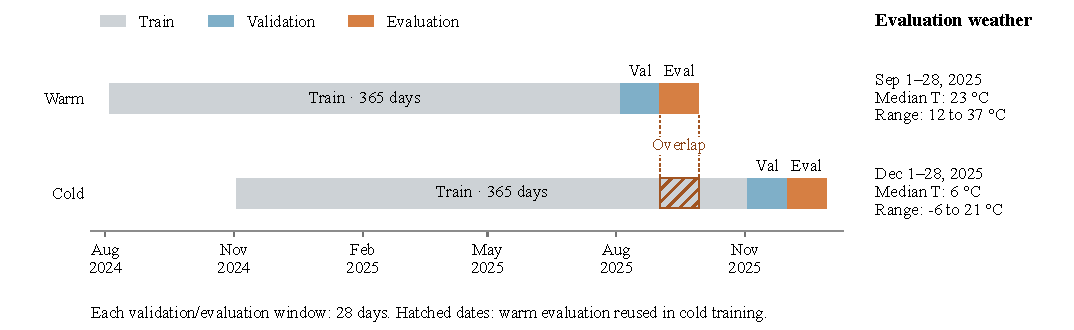
\includegraphics[width=\textwidth]{study_windows.pdf}
\caption{Chronological splits and observed evaluation data. Each split has its own training, validation, and evaluation intervals. Warm evaluation forms part of the cold split's training history, so results are reported separately. Temperature summaries use observed evaluation weather.}
\label{fig:windows}
\end{figure*}

\subsection{Information at the forecast origin}
Each forecast for target hour $t$ uses load history from $[t-168\mathrm{h},t)$. Predictions are generated one hour at a time with fixed model parameters, updating the input history with observations available at each forecast origin.

Missing historical load is reconstructed from earlier observations using weekly lags, same-hour/day-type medians, hour-of-week medians, and a past-observation median, in that order. Reconstructed values are never reused as source observations. The first 31 hours of cold pre-training history have no eligible earlier observation and use zeros with indicators marking the unavailable data; these input-only rows are excluded from scaling and scoring. Training loss and evaluation include observed target loads only.

No observed load values were removed or clipped as outliers during model preparation. Unusually high or low values were retained because the available records do not establish that they are measurement errors. The September exclusion analysis reported below is a separate sensitivity check; those days remain in the primary evaluation.

Missing historical weather is filled with fixed training medians. Load scaling uses observed training targets, whereas weather scaling uses the filled training grid. Calendar inputs comprise cyclic hour, weekday, and hour-of-week encodings, twelve Jalali-month indicators, and working-day, holiday, pre-holiday, and post-holiday indicators. Holidays include Iranian public holidays and Fridays; emergency closures are not independently documented. Historical indicators identify observed load and gaps requiring reconstruction.

\section{Controlled Input Comparisons}
\subsection{Matched information and input removal}
All families receive the same historical and target covariates, with shapes $168\times42$ and $1\times32$. Ridge and XGBoost flatten these tensors into 7,088 columns, preserving duplicated historical weather channels and missingness indicators. No lag selection or additional predictors are introduced. Training-fitted preprocessing and thermal parameters are shared across families within each split.

Table~\ref{tab:conditions} defines the seven conditions. Selected channels are replaced by fixed training medians during fitting and prediction, across all historical and target pathways. Each family is fitted separately under every condition; input dimensions remain fixed. Temperature removal includes its missingness indicator and thermal descendants. Calendar removal affects explicit channels, while reconstructed load can still carry calendar information.

\begin{table}[t]
\caption{Retrained conditions; all retain load history and quality flags}
\label{tab:conditions}
\centering
\footnotesize
\begin{tabular}{@{}p{0.26\columnwidth}p{0.68\columnwidth}@{}}
\toprule
Condition & Change relative to \full \\
\midrule
\full & Raw weather, calendar, and six thermal features. \\
No derived & Replace all six thermal-feature channels. \\
No temperature & Replace temperature, its missing flag, and all thermal features. \\
No humidity & Replace humidity and its missing flag. \\
No calendar & Replace all 22 explicit calendar channels. \\
No weather & Replace temperature, humidity, both missing flags, and thermal features. \\
\proxy & Replace target-hour weather with past-only persistence estimates; retrain. \\
\bottomrule
\end{tabular}
\end{table}


\subsection{TiDE specification and prior design exposure}
\label{sec:model}
TiDE combines dense processing of history and covariates with a horizon-specific decoder and a linear lookback connection \cite{das2023}. The fixed 168-to-1 model has 477,491 parameters: two encoder blocks, one decoder block, hidden width 128, decoder output width 16, temporal projection width 4, temporal hidden width 16, temporal decoder width 32, and dropout 0.1. Reversible instance normalization is disabled. An inherited layer normalization on the scalar temporal-decoder output was replaced by an identity transformation because it removed that branch's input dependence. The other five normalization modules and the lookback connection were retained; the remaining settings were not retuned after this correction.

TiDE uses seeds 42, 314, and 2718, yielding 42 fits. Conditions start from identical weights within each split--seed pair and retain the same parameter count. AdamW uses learning rate $3\times10^{-4}$, weight decay $10^{-4}$, absolute-error loss on scaled load, batch size 64, gradient clipping at 1, and chronological batches. Validation early stopping uses patience 12 and minimum improvement $10^{-4}$. Selected checkpoints are restored without training--validation refitting; neither the 200-epoch nor 30-minute limit is reached.

Earlier experiments screened architectures on 8 October--10 November 2025 and selected the TiDE configuration on 11--26 November. The thermal-feature family was subsequently selected on the same intervals with the corrected model. Warm evaluation dates had appeared in earlier training data. In cold evaluation, 1--21 December had served as ensemble validation, 22 December as context, and 23--28 December as test data. These periods are therefore not previously unseen holdouts. The cross-family comparison was designed after inspecting TiDE results, with its search and analysis rules fixed before scoring the new evaluation predictions.

\subsection{Regularized linear and boosted-tree models}
Ridge-ARX predicts load in kW using an intercept and all flattened predictors, minimizing the residual sum of squares plus an $L_2$ coefficient penalty. Its penalty is selected from $\{0.01,0.1,1,10,100,1000,10000\}$; warm and cold selections are 100 and 10. The solution is deterministic, giving 14 final fits rather than replicated seed runs.

XGBoost uses squared-error loss on load measured in kW and histogram-based trees with up to 64 bins. Twelve prespecified candidates per split vary depth, learning rate, minimum child weight, row and column sampling, and $L_2$ regularization. Selection uses seed 42. Both splits select learning rate 0.03; warm/cold settings are depth 4/2, minimum child weight 5/1, row sampling 0.8/1, column sampling 1/0.6, and $L_2$ penalty 10/1. Early stopping monitors validation MAE with patience 50 and a ceiling of 2,000 rounds. Seven final cold fits reach that ceiling; the best validation iteration is retained, without assuming convergence.

For each new family and split, hyperparameters are selected using \full\ training and observed-target validation MAE, then held fixed across conditions. XGBoost tree counts may vary by condition and seed under the same stopping rule. Seeds 42, 314, and 2718 give 42 final XGBoost fits. All models use training targets only, without refitting on training plus validation. TiDE predictions are reused unchanged. For TiDE and XGBoost, ensemble forecasts average the three predictions in kW before scoring; individual fits are also assessed. Ridge remains a single fitted predictor. Matching inputs does not equate optimization objectives, capacity, or tuning budgets.

\subsection{Thermal representation}
For temperature $T_s$, heating and cooling excess are
\begin{equation}
H_s=\max(\theta_h-T_s,0),\qquad
C_s=\max(T_s-\theta_c,0).
\label{eq:excess}
\end{equation}
Four further features sum these quantities over the preceding 6 or 24 hours. With hourly indices $s\in\{t-168,\ldots,t\}$,
\begin{equation}
A^H_{k,s;t}=\sum_{u=\max(t-168,\,s-k)}^{s-1}H_u,
\quad k\in\{6,24\},
\label{eq:accum}
\end{equation}
with an analogous cooling sum and zero for an empty sum. Each sum excludes the feature's current hour and stops at the beginning of the forecast's history. Early historical sums are truncated; target-hour sums use all $k$ preceding hours. The representation thus has two excess and four degree-hour features.

Threshold selection uses an auxiliary Ridge model, distinct from the 7,088-column comparator: penalty 10, load lags 1, 24, and 168 hours, and calendar controls. Four expanding training prefixes ending on days 181, 227, 273, and 319 are followed by 46-day inner validation intervals. Selection minimizes their equally weighted mean daily WAPE, with preprocessing refitted in each prefix. Heating candidates are 10, 14, 18, and 22\degc; cooling candidates are 18, 22, 26, and 30\degc, with $\theta_h\leq\theta_c$. Each candidate needs at least 100 jointly observed load--temperature samples on each side of each threshold in every prefix.

The selected pairs, shared by all model families, are $(10,18)$\degc\ for warm and $(10,22)$\degc\ for cold. Both heating thresholds and the warm cooling threshold lie at the lower grid boundary; cold cooling candidates above 22\degc\ lack training support. Small runner-up gaps also limit identification. These are grid-constrained predictive parameters, not physical balance temperatures. Thermal scaling includes repeated appearances within training windows but excludes pre-training rows.

\subsection{Realized weather and persistence proxy}
The main ablations use realized target-hour weather for retained channels. In \proxy, target temperature and humidity are estimated separately from their latest observations in $[t-168\mathrm{h},t)$, with a training-median fallback. Target missingness indicators reflect the availability of an earlier observation, not actual target-hour missingness. Historical weather is unchanged and target thermal features are recomputed. Every family trains \proxy\ separately, using the same thresholds and preprocessing as its \full\ condition.

No fallback is needed in validation or evaluation. Evaluation donors are typically one hour old, with maxima of four hours warm and two hours cold. The proxy usually repeats weather already present in the history, placing past-based estimates in the target inputs without supplying a new observation. It retains historical weather, unlike the all-weather ablation. Archived weather forecasts and a complete set of ablations under restricted weather access are not evaluated.

\subsection{Error measures and paired comparisons}
For observed targets $O_d$ on day $d$, daily weighted absolute percentage error and its mean are
\begin{equation}
W_d=100\frac{\sum_{t\in O_d}|\hat y_t-y_t|}{\sum_{t\in O_d}|y_t|},
\qquad \mdw=\frac{1}{D}\sum_{d=1}^{D}W_d.
\label{eq:wape}
\end{equation}
All 28 days enter the primary score, including incomplete days. Pooled WAPE aggregates numerator and denominator across the window. Simple references predict load recorded 1, 24, or 168 hours earlier, using the same causal reconstruction when missing and the same observed targets. MAE, RMSE, and mean signed bias $\hat y_t-y_t$ are in kW. Peak-magnitude error is $|\max_t\hat y_t-\max_t y_t|$ on complete days; peak timing uses the absolute hour difference between the earliest maxima. Peak comparisons are descriptive, without confidence intervals.

Within each family, define $\Delta_a=\mdw_a-\mdw_{\full}$ for condition $a$, in percentage points (pp). Positive values favor \full. No weather and no temperature are the primary contrasts; other removals, \proxy, and direct family rankings are supplementary. Paired daily differences use noncircular three-day moving-block bootstrap resampling with 10,000 draws, seed 20260926, and 95\% percentile limits. Intervals condition on fixed fitted models or ensembles and dates; they exclude retraining uncertainty and are not multiplicity-adjusted. Matched seed-level differences separately describe training variability for TiDE and XGBoost.

\section{Results}
\subsection{Input value across model families and periods}
Table~\ref{tab:results} reports all seven conditions. Among the matched-information \full\ configurations, mean daily WAPE is 5.91\% warm and 5.86\% cold for TiDE ensembles, 6.58\% and 6.95\% for XGBoost ensembles, and 7.11\% and 7.44\% for Ridge. All three improve on the warm persistence references. In cold evaluation, the previous-day reference (6.84\%) outperforms Ridge and XGBoost \full, although their no-weather conditions improve on it. These scores describe the fitted configurations rather than a general ranking of architectures; ensemble and individual-fit performance are distinguished below.

\begin{table*}[t]
\caption{Evaluation mean daily WAPE (\%). Ridge-ARX is deterministic; XGBoost and TiDE use the mean prediction of three seeds. Each window contains 28 days and 626 (warm) or 669 (cold) observed targets. Persistence references use the same reconstructed history and observed targets.}
\label{tab:results}
\centering
\begin{tabular}{@{}lrrrcrrr@{}}
\toprule
& \multicolumn{3}{c}{Warm} && \multicolumn{3}{c}{Cold}\\
\cmidrule(lr){2-4}\cmidrule(l){6-8}
Condition & Ridge-ARX & XGBoost & TiDE && Ridge-ARX & XGBoost & TiDE\\
\midrule
\full & 7.11 & 6.58 & 5.91 && 7.44 & 6.95 & 5.86\\
No derived & 6.90 & 6.64 & 6.25 && 5.43 & 7.08 & 5.49\\
No temperature & 6.75 & 6.91 & 6.21 && 5.12 & 6.08 & 4.98\\
No humidity & 6.96 & 6.47 & 5.60 && 7.25 & 7.07 & 4.97\\
No calendar & 6.84 & 6.88 & 5.88 && 5.90 & 6.73 & 5.34\\
No weather & 6.52 & 6.83 & 6.22 && 4.98 & 5.99 & 5.07\\
\proxy & 7.18 & 6.59 & 6.20 && 7.57 & 6.66 & 5.19\\
\midrule
Previous hour & \multicolumn{3}{c}{8.61} && \multicolumn{3}{c}{8.36}\\
Previous day & \multicolumn{3}{c}{13.01} && \multicolumn{3}{c}{6.84}\\
Previous week & \multicolumn{3}{c}{35.13} && \multicolumn{3}{c}{12.24}\\
\bottomrule
\end{tabular}
\end{table*}


\begin{figure*}[t]
\centering
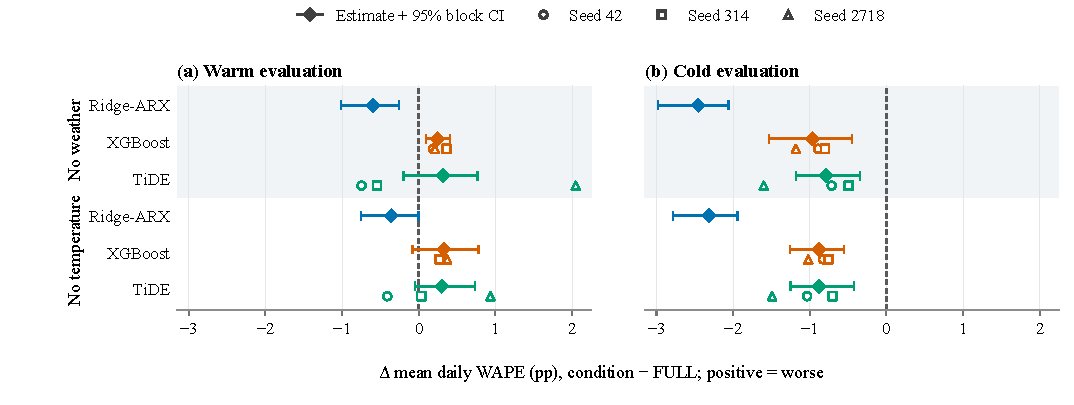
\includegraphics[width=\textwidth]{i15_primary_value.pdf}
\caption{Primary evaluation contrasts relative to each family's \full. Filled estimates show deterministic Ridge or three-seed prediction ensembles; open markers show individual stochastic fits. Bars are conditional, unadjusted 95\% paired three-day block intervals. Positive values favor \full.}
\label{fig:paired}
\end{figure*}

Cold evaluation gives a consistent direction across families (Fig.~\ref{fig:paired}). Removing all weather lowers mean daily WAPE by 2.45 pp for Ridge, 0.97 pp for XGBoost, and 0.79 pp for TiDE, with intervals $[-2.98,-2.06]$, $[-1.53,-0.45]$, and $[-1.18,-0.34]$. Temperature removal also lowers error: by 2.32, 0.88, and 0.88 pp, respectively, with all three intervals below zero. Ridge's no-weather condition improves every one of the 28 daily scores. The direction is therefore not confined to the dense neural model.

Warm evaluation separates the families. Weather removal helps Ridge by 0.59 pp (interval $[-1.01,-0.26]$) but harms XGBoost by 0.25 pp ($[0.10,0.41]$). TiDE's ensemble difference is $+0.32$ pp ($[-0.20,0.77]$), with seed disagreement. Temperature-removal point estimates have the same family-specific directions: $-0.36$, $+0.33$, and $+0.30$ pp for Ridge, XGBoost, and TiDE. The latter two intervals include zero; Ridge's upper limit is essentially zero, making this contrast borderline. Thus, the evidence for warm weather value is family-specific, not a shared benefit or penalty.

\begin{table}[t]
\caption{Changes in mean daily WAPE relative to \full\ (pp). W: no weather; T: no temperature. Val: validation; Eval: evaluation. Positive differences favor \full; $+0.00$ denotes a rounded positive value.}
\label{tab:contrasts}
\centering
\footnotesize
\setlength{\tabcolsep}{3pt}
\begin{tabular}{@{}llrrrr@{}}
\toprule
&& \multicolumn{2}{c}{Warm} & \multicolumn{2}{c}{Cold}\\
\cmidrule(lr){3-4}\cmidrule(l){5-6}
Model & Removed & Val & Eval & Val & Eval\\
\midrule
Ridge-ARX & W & $-0.36$ & $-0.59$ & $-1.52$ & $-2.45$\\
 & T & $-0.21$ & $-0.36$ & $-1.46$ & $-2.32$\\
XGBoost & W & $+0.21$ & $+0.25$ & $-0.47$ & $-0.97$\\
 & T & $+0.27$ & $+0.33$ & $-0.08$ & $-0.88$\\
TiDE & W & $-0.02$ & $+0.32$ & $+0.06$ & $-0.79$\\
 & T & $+0.05$ & $+0.30$ & $+0.00$ & $-0.88$\\
\bottomrule
\end{tabular}
\end{table}


Validation provides a further check (Table~\ref{tab:contrasts}). For deterministic Ridge and the XGBoost ensembles, all eight primary point-estimate contrasts retain their direction from validation to evaluation: two removals in each window for each family. This agreement concerns direction, not significance in every comparison. Cold weather removal already favors Ridge and XGBoost in validation, by 1.52 and 0.47 pp. TiDE's corresponding difference is $+0.06$ pp, close to zero, before becoming negative in evaluation. The lack of a validation advantage for cold weather removal is consequently specific to TiDE. Changes in load level could alter learned input relationships, but these comparisons do not identify the mechanism.

\subsection{Training variability and the September load change}
In evaluation, all three seeds of both stochastic families favor cold temperature and weather removal. Warm XGBoost evaluation also has consistent signs: removing either input raises error in every seed. Warm TiDE does not: weather-removal differences are $-0.75$, $-0.54$, and $+2.05$ pp for seeds 42, 314, and 2718. Its positive ensemble difference therefore does not indicate agreement among individual fits. Under warm \full, TiDE's individual-fit mean WAPE is 6.55\% with sample standard deviation 0.43 pp, whereas its prediction ensemble scores 5.91\%. The ensemble benefit is not evidence that every TiDE fit outperforms XGBoost.

A descriptive TiDE leave-one-seed-out check changes the warm weather-removal contrast from $+0.32$ to $-0.28$ pp when seed 2718 is omitted; all three two-seed cold contrasts remain negative. These checks diagnose sensitivity without replacing the specified ensemble.

The existing TiDE sensitivity analysis excludes 23--27 September from scoring, leaving 23 days and 507 observed targets without refitting. Warm \full\ WAPE falls from 5.91\% to 4.77\%, while weather- and temperature-removal differences remain positive at $+0.51$ and $+0.33$ pp. All six contrasts still have mixed seed signs. This post-hoc check was not extended to the new families; the primary analysis retains every day. WAPE can rise when the load denominator falls even without a proportional rise in absolute error.

\subsection{Other input groups and weather availability}
Humidity, calendar, and thermal results also vary by family. Cold humidity removal lowers WAPE by 0.19 pp for Ridge and 0.89 pp for TiDE but raises it by 0.12 pp for XGBoost; the respective intervals exclude zero. Removing thermal features lowers cold error for Ridge and TiDE but gives XGBoost a small increase whose interval includes zero. For Ridge, the reduction is 2.01 pp, from 7.44\% to 5.43\%. Warm calendar-removal intervals include zero in all families. These effects concern explicit inputs conditional on the remaining information, and cannot be added into a decomposition of demand.

Thermal activation differs across windows: heating quantities are zero throughout warm evaluation inputs, while cold target-hour cooling quantities are zero, with nonzero historical cooling confined to the first 63 origins. The six-channel removal therefore compares different activation patterns and training histories, not equivalent physical heating and cooling effects.

The persistence proxy is also model-dependent. Cold \proxy\ changes WAPE by $+0.13$ pp for Ridge, $-0.29$ pp for XGBoost, and $-0.66$ pp for TiDE, with intervals above, below, and below zero, respectively. Warm differences are $+0.07$, approximately zero, and $+0.29$ pp. These comparisons reflect both weather availability and adaptation of separately fitted models. They do not establish that persistence weather is generally better than observed weather or than an operational forecast.

\subsection{Average and peak forecasting performance}
Fig.~\ref{fig:tradeoff} shows that the relation between average and peak errors depends on the model. Cold weather removal reduces mean daily WAPE in every family, yet peak-magnitude MAE falls by 1105.8~kW for Ridge and 1798.4~kW for XGBoost while rising by 433.5~kW for TiDE. TiDE's peak error increases from 2739.99 to 3173.52~kW (15.8\%). Its peak timing improves from 1.76 to 1.48 hours, whereas XGBoost's worsens from 1.96 to 2.16 hours and Ridge's remains at 1.64 hours.

\begin{figure}[t]
\centering
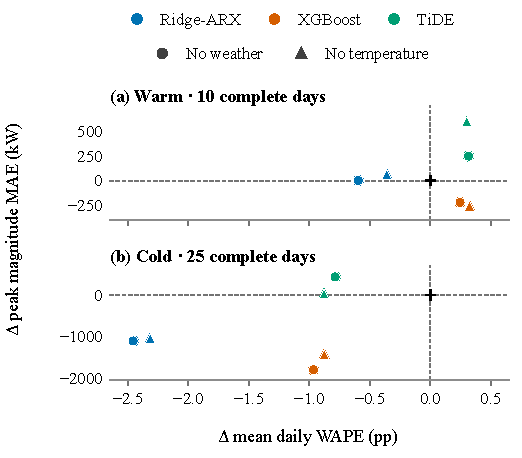
\includegraphics[width=\columnwidth]{i15_mean_peak_tradeoff.pdf}
\caption{Evaluation changes in mean daily WAPE and peak-magnitude MAE after weather or temperature removal. Lower is better on both axes; the cross marks \full. Vertical scales differ. Peaks use 10 warm and 25 cold complete days; WAPE uses all 28 days. Ridge is deterministic; other points use prediction ensembles. Peak differences are descriptive.}
\label{fig:tradeoff}
\end{figure}

Warm XGBoost weather removal gives the opposite trade-off: mean error increases by 0.25 pp while peak-magnitude MAE falls by 219.6~kW. Thus, an input choice based on mean error need not minimize either peak magnitude or timing error. Peak comparisons have no quantified uncertainty and use fewer days than mean daily WAPE, particularly in the warm window; they reflect both different objectives and different observation support.

\section{Discussion and Limitations}
The cold reduction in mean error after weather removal is consistent across a linear model, boosted trees, and a dense neural model sharing the same inputs, preprocessing, thermal thresholds, and windows. These comparisons do not provide independent replications. Warm disagreement and contrasting peak responses show that useful inputs depend on the model, period, and objective. These results accord with earlier reports of limited or model-dependent weather gains \cite{haben2019,yang2024}, while recent load can already carry weather and calendar information.

The humidity results concern additional forecasting information, not a physical absence of humidity sensitivity. They do not contradict improvements from heat-stress measures in monthly demand models \cite{maia2020}, which use different targets and representations. Temperature preprocessing and recency studies \cite{candela2022,wang2016} motivate testing thermal memory, but do not establish that the present thresholds or 6- and 24-hour sums are optimal. No condition removes load history, and calendar-informed reconstruction remains even when explicit calendar channels are masked.

For input selection, agreement across validation and evaluation, seed stability, and peak performance matter alongside the mean score. The load-level changes also motivate monitoring bias and testing recalibration fitted only on past data. The present experiments neither identify the cause of those changes nor show that recalibration would resolve them.

Three model families do not remove the limits of two short, previously inspected windows. Warm evaluation lies within cold training, and differences in histories, missingness, and fitted thresholds prevent attributing changes solely to season. The new comparisons followed inspection of TiDE results. Objectives and tuning budgets differ, and the high-dimensional representation is held fixed rather than optimized for each family. Using \full-selected hyperparameters controls the tuning choice across removals, but does not establish the best regularization or tree settings for each reduced-input condition. In particular, Ridge's preferred penalty may change when correlated predictor groups are masked. Seven final cold XGBoost fits reach the training ceiling; sensitivity to a higher ceiling was not assessed, so longer training could change the comparisons. Direct rankings therefore apply to these fitted configurations. Three seeds provide limited evidence about training variability; day-bootstrap intervals are conditional and unadjusted.

Missing warm-weather records and incomplete spatial metadata restrict physical interpretation. Only \proxy\ restricts retained target-weather channels to earlier observations; other weather-containing conditions use realized values. Previously unused chronological periods, archived weather forecasts, and matched-budget model tuning are needed to assess transfer. The present evidence concerns conditional predictive value, not causal contributions to consumption.

\section{Conclusion}
With 168 hours of load history, removing temperature or all weather lowers cold-window mean daily WAPE in Ridge-ARX, XGBoost, and TiDE. Warm effects differ across families and are unstable across TiDE seeds. The cold mean-error agreement also does not extend to peak magnitude: removal improves Ridge and XGBoost peak errors but worsens TiDE's. Input selection should therefore be evaluated across model families, periods, training runs, and forecast objectives. These retrospective findings support conditional input assessment; independent temporal evaluation with realistic weather availability is required before treating the observed rankings as transferable.

\section*{Acknowledgment}
OpenAI ChatGPT and Codex assisted with drafting and revising text throughout the manuscript, organizing and debugging code, preparing analysis and figure-generation code, and editing LaTeX. Anthropic Claude assisted with manuscript critique and verification of reported results. These tools supported preparation rather than providing independent scientific evidence. The authors are responsible for the study design, verification of the analyses and references, interpretation of the results, and final manuscript.

% Balance final columns while preserving bibliography reading order.
\balance
\bibliographystyle{IEEEtran}
\bibliography{references}
\end{document}
